% <!-- coding: utf-8 -->
% http://www.cosmosportal.eu/cosmos/files/help/interactive_pdfs.pdf
\documentclass[a4paper,twoside,english]{article}
% \usepackage{minitoc}
\usepackage[utf8]{inputenc}
\usepackage[T1]{fontenc}
\usepackage[frenchb]{babel}
\usepackage{lmodern}% Choix de la fonte (Latin Modern de D. Knuth) %
\usepackage{textcomp} % pour l'euro
\usepackage{datetime}
% http://en.wikibooks.org/wiki/LaTeX/Page_Layout
% http://www.tex.ac.uk/tex-archive/info/apprends-latex/Apprends_LaTeX.pdf
\usepackage[top=2cm, bottom=2cm, left=0.5cm, right=0.5cm]{geometry}
% \DeclareGraphicsExtensions{.jpg,.mps,.pdf,.png} % Formats d'images
%
% mes personnalisations pour le document
\newcommand{\montitre}{Bretagne Vivante Rennes - Vilaine Aval}
\newcommand{\monlhead}{Bretagne Vivante Rennes - Vilaine Aval}
\newcommand{\malargeurgraphique}{93mm}
% les espaces en fin de ligne
\frenchspacing
% pour la planche contact
% http://en.wikibooks.org/wiki/LaTeX/Floats,_Figures_and_Captions
% \usepackage[demo]{graphicx}
\usepackage{graphicx}
\usepackage{caption}
%
\usepackage{subcaption}
% http://www.peteryu.ca/tutorials/publishing/latex_captions
\captionsetup[subfigure]{labelformat=empty}
% pour supprimer la numérotation
% \renewcommand{\thesubfigure}{\arabic{subfigure}}
\renewcommand{\thesubfigure}{}
%
% la séparation entre les figures
% http://newsgroups.derkeiler.com/Archive/Comp/comp.text.tex/2010-08/msg00435.html
\setlength{\textfloatsep}{0pt}
\setlength{\floatsep}{0pt}
% la date en francais
\usepackage{datetime}
\newdateformat{mydate}{\THEDAY/\THEMONTH/\THEYEAR}
%
% la personnalisation des entête/pied de page
\usepackage{fancyhdr}
\usepackage{lastpage}
\fancyhf{}
\fancyhead[LO,RE]{\fontsize{14}{16}\selectfont\monlhead}
\fancyhead[LE,RO]{\fontsize{14}{16}\selectfont\montitre}
\pagestyle{fancy}
\renewcommand\sectionmark[1]{\markboth{\MakeUppercase{#1}}{}}
\rfoot{\thepage/\pageref{LastPage}}
\cfoot{Matthieu Beaufils \& Marc Gauthier}
\lfoot{\mydate\today}
% on supprime la ligne en dessous de l'entête
\renewcommand{\headrulewidth}{0pt}

%
% pour les deux colonnes
\usepackage{supertabular}
%
% pour les trois colonnes
\usepackage{multicol}
% pour améliorer les tableaux
\usepackage{array}
%

% http://tex.stackexchange.com/questions/66252/placing-the-figure-exactly-at-the-top-of-the-page-in-latex
\makeatletter
\setlength{\@fptop}{0pt}
\makeatother
% http://tex.stackexchange.com/questions/42968/reduction-of-space-between-two-sub-figures
% \usepackage{showframe}
%
% pour les tables des matières
% http://tex.stackexchange.com/questions/186515/remove-chapter-number-from-minitoc
% \newcommand{\filterminitoc}[1]{#1}
% \renewcommand{\thesection}{\csname filterminitoc \endcsname{\arabic{chapter}.}\arabic{section}}
% \newcommand{\minitocsection}{\begingroup\renewcommand{\filterminitoc}[1]{}\minitoc\endgroup}
\newcommand{\HRule}{\rule{\linewidth}{0.5mm}}
% pour les carrés de couleur
\usepackage{xcolor}

\usepackage{titlesec}
\titlespacing*{\subsubsection}{0pt}{5pt}{0pt}
\usepackage{hyperref}
\hypersetup{
   pdfauthor   = {Marc Gauthier},
   colorlinks=true,
   breaklinks=true,
   urlcolor= blue,
   linkcolor= blue,
   linkbordercolor=blue,
   pdfcreator  = {\LaTeX},
}
\newcommand\crule[3][black]{\textcolor{#1}{\rule{#2}{#3}}}
% les espaces en fin de ligne
\frenchspacing
% http://daniel.flipo.free.fr/frenchb/frenchb-doc.pdf
% http://borntocode.fr/latex-customisation-de-listes-a-puces/
% https://en.wikibooks.org/wiki/LaTeX/List_Structures
% \frenchbsetup{StandardItemizeEnv=true, StandardEnumerateEnv=true, ReduceListSpacing=true, ItemLabels=\textendash}
% pour avoir les versions des modules
\listfiles
\begin{document}
%
% la page de garde
% http://www.jujens.eu/posts/2013/Oct/20/latex-page-garde/
\begin{titlepage}
  \begin{sffamily}
  \begin{center}

    % Upper part of the page. The '~' is needed because \\
    % only works if a paragraph has started.


    \textsc{\LARGE Bretagne Vivante Rennes}\\[1cm]
    \textsc{\Large Vilaine Aval - oiseaux en hiver}\\[1cm]

    % Title
    \HRule \\[0.4cm]
    { \huge \bfseries Données faune-bretagne}
    \HRule \\[0.4cm]
    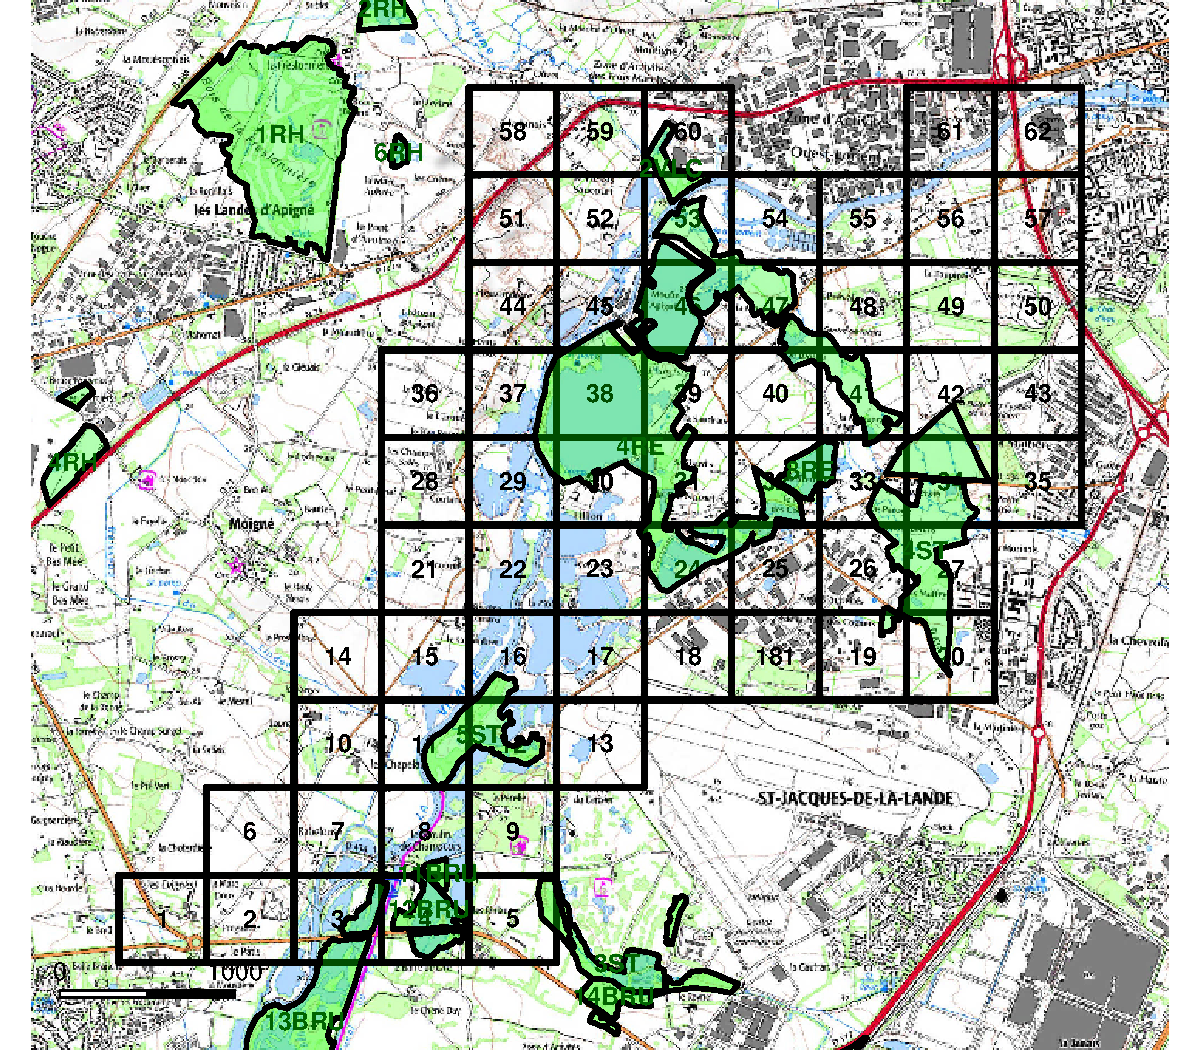
\includegraphics[width=190mm]{territoire_Nord.pdf}~\\[.5cm]
    \HRule \\[0.4cm]
    \begin{minipage}{0.4\textwidth}
      \begin{flushleft} \large
        \emph{Coordination}\\
        Matthieu Beaufils\\
         Marc Gauthier
      \end{flushleft}
    \end{minipage}
    \begin{minipage}{0.4\textwidth}
      \begin{flushright} \large
        \emph{Informatique}\\
        Marc Gauthier
      \end{flushright}
    \end{minipage}

    \vfill
  \end{center}
  \end{sffamily}
\end{titlepage}
\setlength{\parskip}{0pt} % 1ex plus 0.5ex minus 0.2ex}
\setlength{\parindent}{0pt}
\twocolumn
% <!-- coding: utf-8 -->
\renewcommand{\monlhead}{Données ornitho faune-bretagne}
\section*{Présentation}
Les données sont extraites de faune-bretagne sur la zone géographique -1.775795/48.105037 -1.711859/48.060601

Cette extraction est faite en format csv. Les données sont ensuite traitées en R

Un rapprochement est effectué avec le référenciel taxonomique TAXREF.
Les espèces spécifiques à biolovision ne sont pas prises en compte.

Les familles sont différentes pour certaines espèces, en version 9.0 de TAXREF :
\begin{itemize}
\item Roitelet à triple bandeau   Sylviidae   Regulidae
\item Rougegorge familier    Turdidae Saxicolidae
\end{itemize}

Des statistiques sont produites pour :
\begin{itemize}
\item les données sur la zone d'extraction
\item les données sur la période 1er décembre 2016 - 20 janvier 2017
\end{itemize}
\section*{Statistiques données antérieures}
\subsection*{par famille}
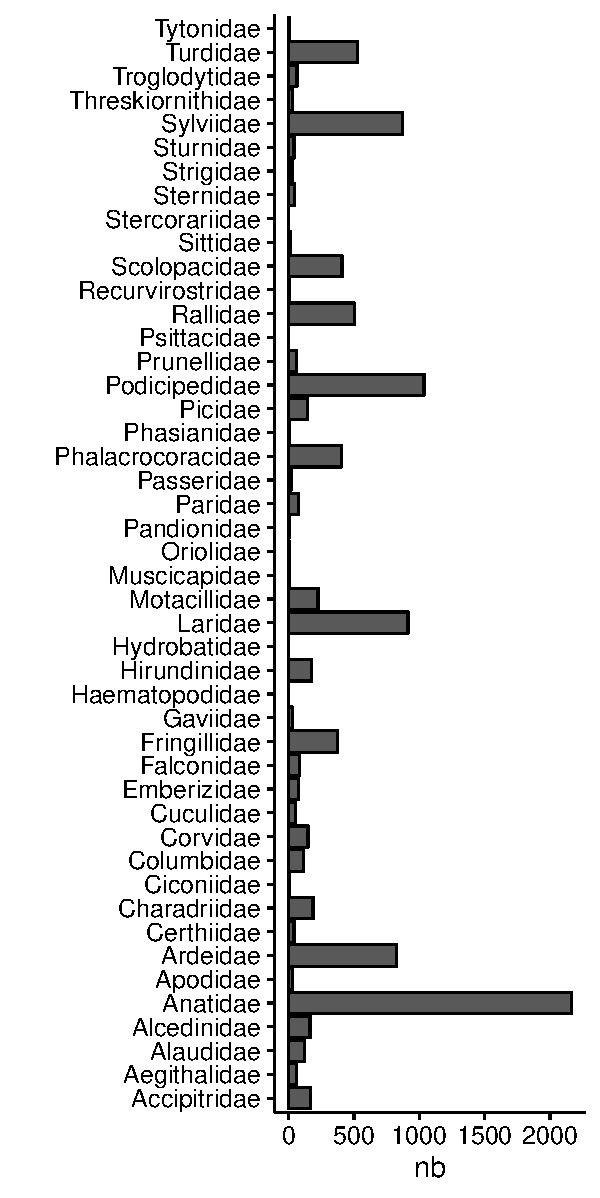
\includegraphics[width=\malargeurgraphique]{images/faune_prec_stat_champ_FAMILY_NAME.pdf}
\subsection*{par année}
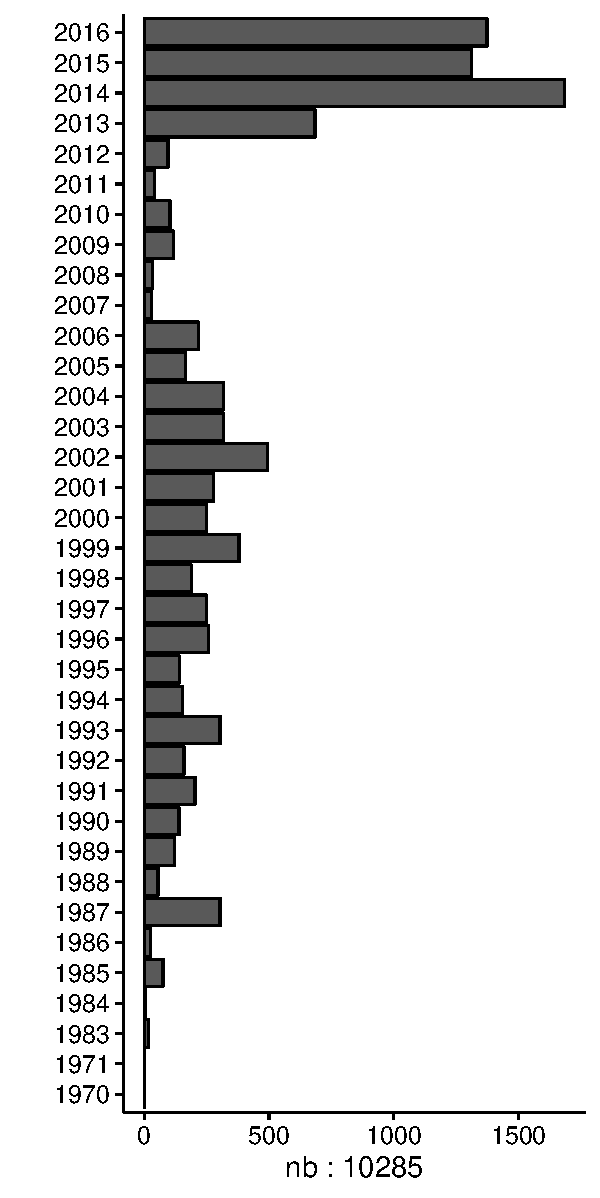
\includegraphics[width=\malargeurgraphique]{images/faune_prec_stat_champ_annee.pdf}
\subsection*{par mois}
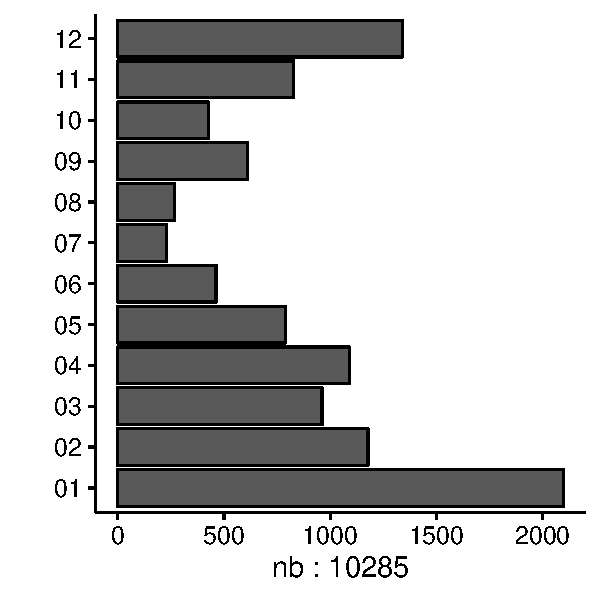
\includegraphics[width=\malargeurgraphique]{images/faune_prec_stat_champ_mois.pdf}
\subsection*{par type de localisation}
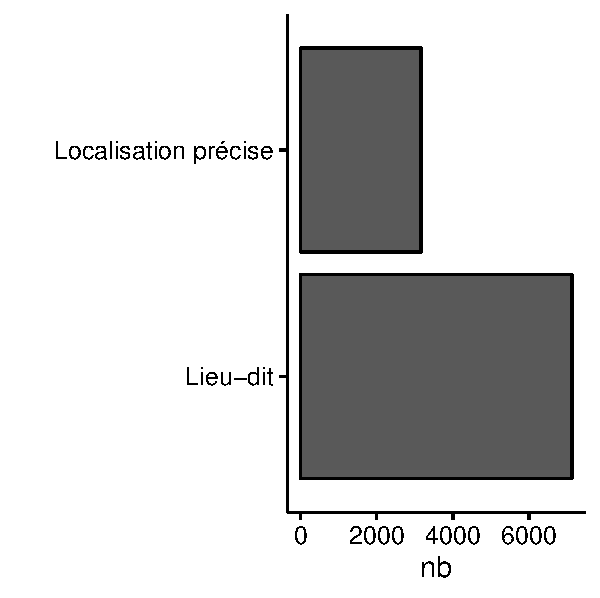
\includegraphics[width=\malargeurgraphique]{images/faune_prec_stat_champ_PRECISION.pdf}
\section*{Statistiques 1er décembre 2016 - 20 janvier 2017}
\subsection*{par famille}
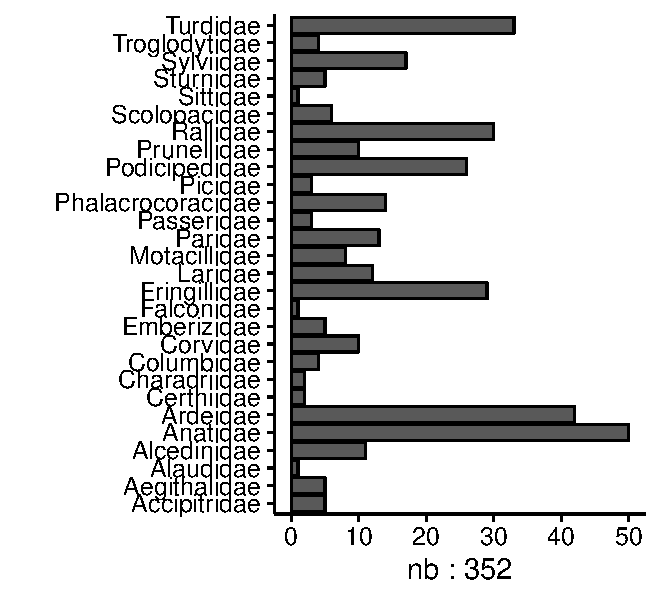
\includegraphics[width=\malargeurgraphique]{images/faune_stat_champ_FAMILY_NAME.pdf}
\subsection*{par famille taxref}
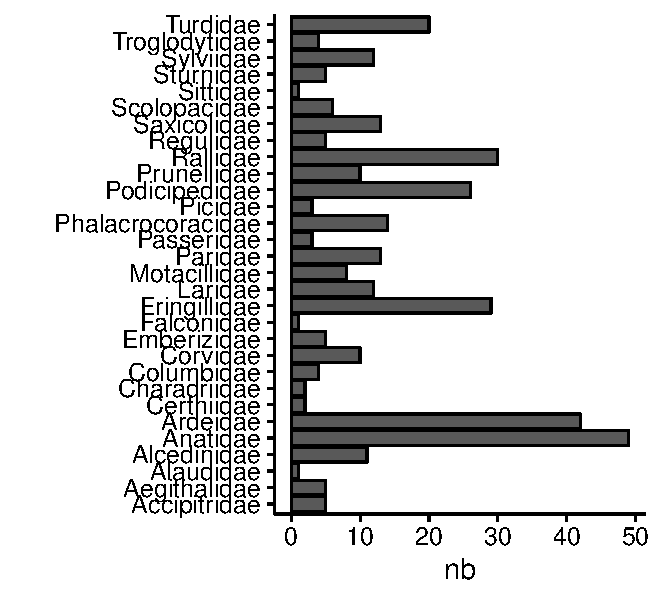
\includegraphics[width=\malargeurgraphique]{images/faune_stat_champ_FAMILLE.pdf}
\subsection*{par ordre taxref}
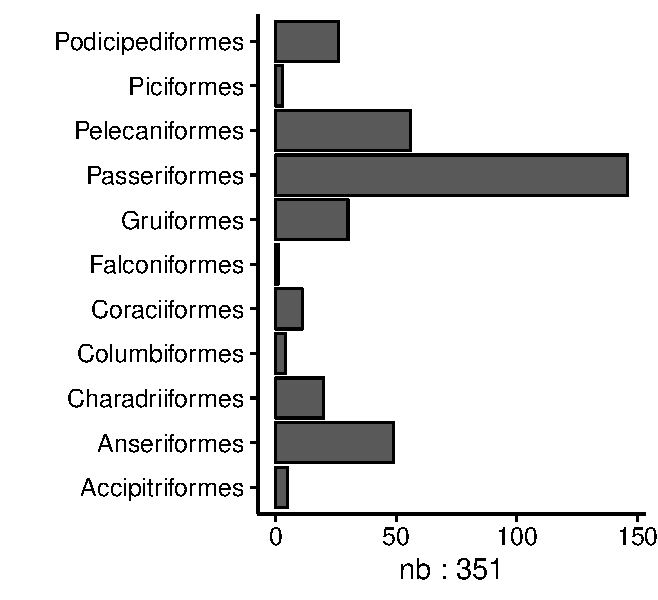
\includegraphics[width=\malargeurgraphique]{images/faune_stat_champ_ORDRE.pdf}
\subsection*{par espèce}
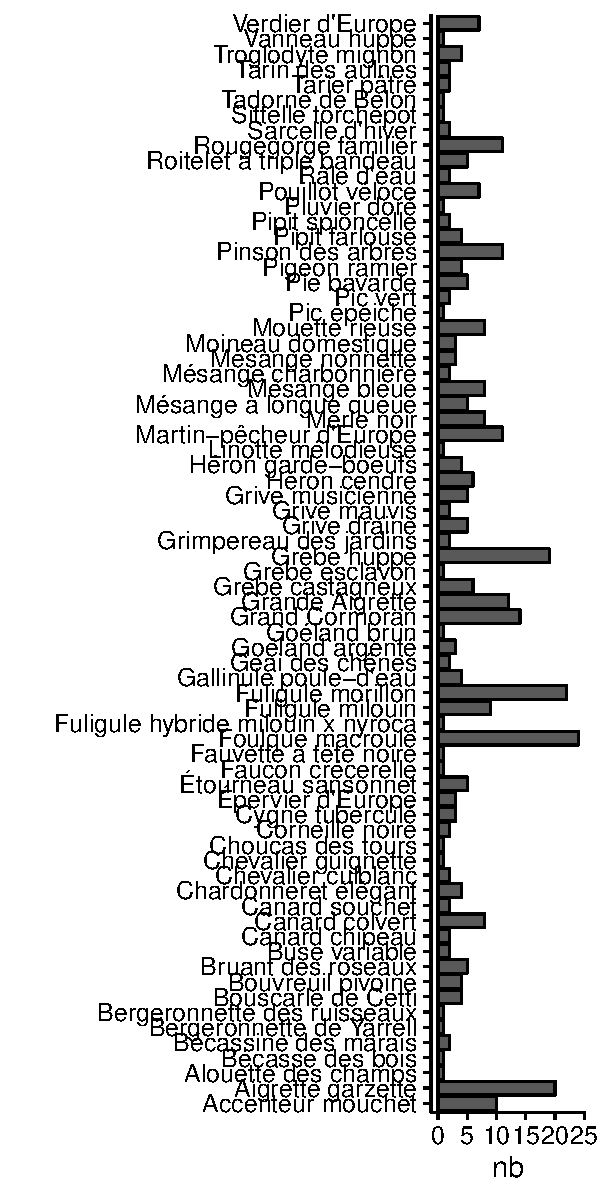
\includegraphics[width=\malargeurgraphique]{images/faune_stat_champ_NAME_SPECIES.pdf}
\subsection*{par date}
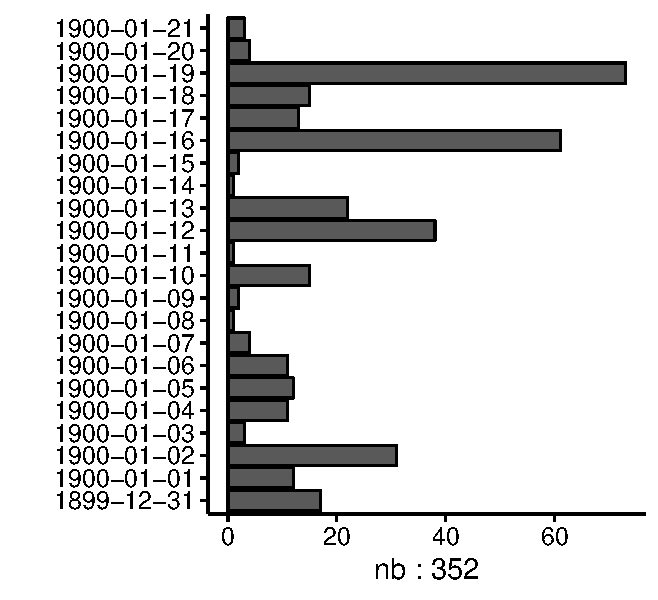
\includegraphics[width=\malargeurgraphique]{images/faune_stat_champ_d.pdf}
\subsection*{par observateur}
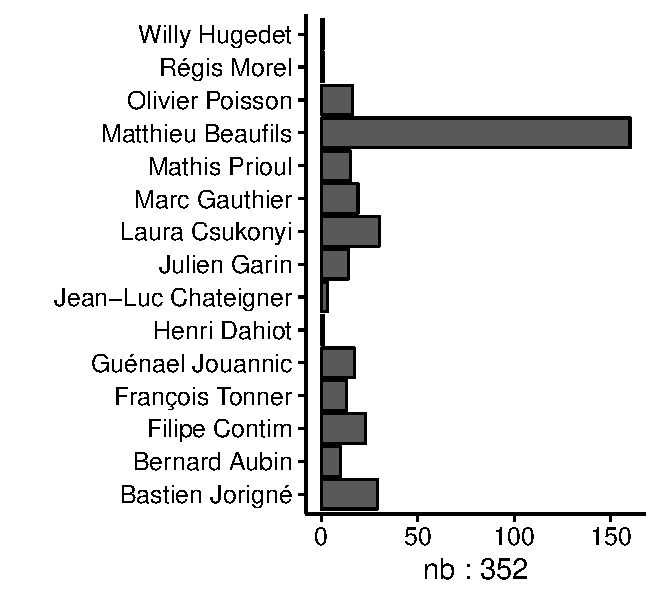
\includegraphics[width=\malargeurgraphique]{images/faune_stat_champ_observateur.pdf}
\subsection*{par lieudit}
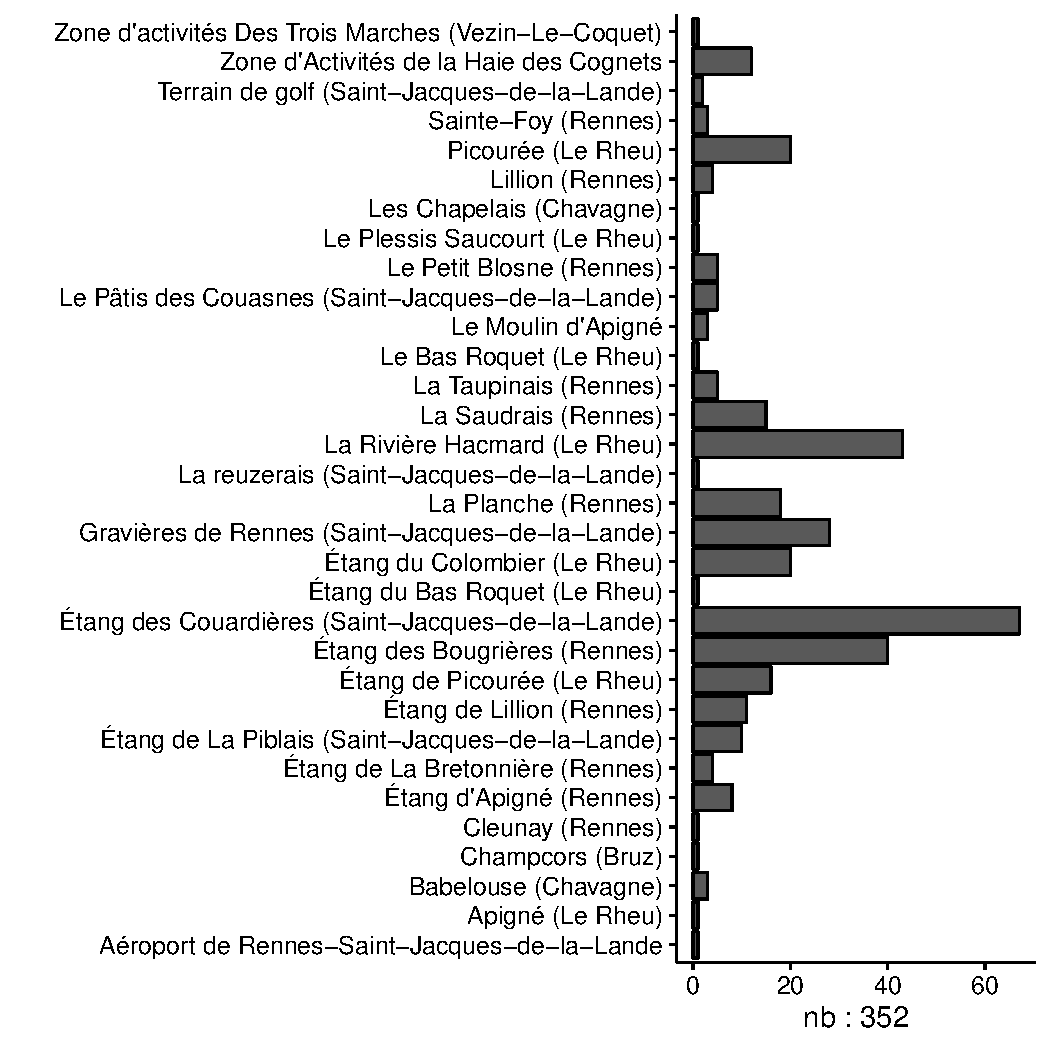
\includegraphics[width=\malargeurgraphique]{images/faune_stat_champ_PLACE.pdf}
\subsection*{par type de localisation}
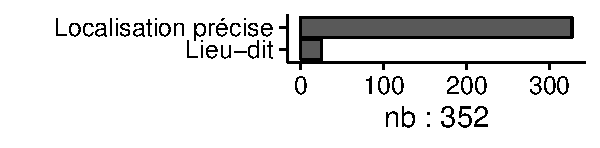
\includegraphics[width=\malargeurgraphique]{images/faune_stat_champ_PRECISION.pdf}
\clearpage
\section*{Carte}
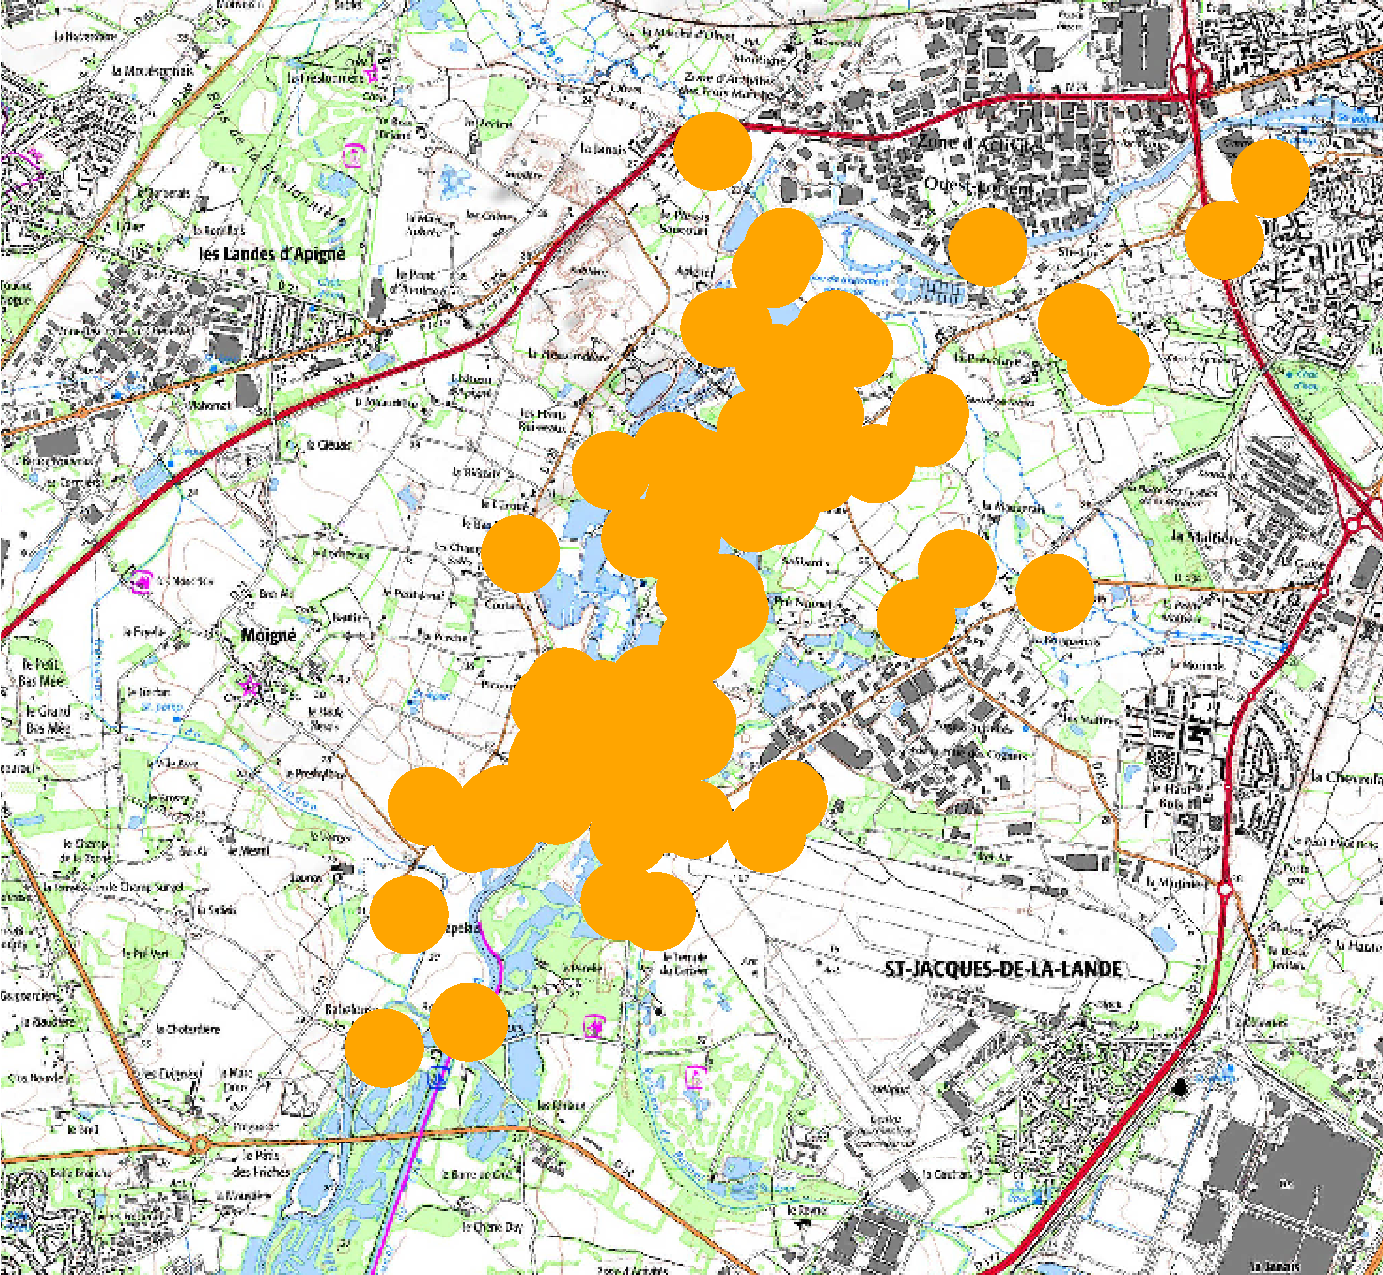
\includegraphics[width=\textwidth]{images/faune_carte.pdf}
\onecolumn
\end{document}